%% Computers & Security (Elsevier) submission
%% Compile on Overleaf with pdfLaTeX: main.tex -> BibTeX -> pdfLaTeX x2
\documentclass[preprint,11pt,authoryear]{elsarticle}

\usepackage[T1]{fontenc}
\usepackage[utf8]{inputenc}
\usepackage{graphicx}
\usepackage{booktabs}
\usepackage{amsmath}
\usepackage{amssymb}
\usepackage{algorithm}
\usepackage{algpseudocode}
\usepackage{multirow}
\usepackage{url}
\usepackage[hidelinks]{hyperref}
\usepackage{siunitx}
\sisetup{detect-all, per-mode=symbol}

\journal{Computers \& Security}

\newcommand{\phirel}{\phi^{\mathrm{rel}}}
\newcommand{\phires}{\phi^{\mathrm{res}}}
\newcommand{\FA}{\mathrm{FA}}

\begin{document}

\begin{frontmatter}

\title{Deployable Intrusion Detection for the CAN Bus: An Event-Level Evaluation
Protocol and Identifier-Agnostic Detectors that Transfer Across Vehicles}

\author[a]{First Author}
\ead{author@univ.edu}
\author[a]{Second Author}
\author[a]{Third Author}
\affiliation[a]{organization={Department of Computer Science and Engineering, University XXXX},
                city={City}, country={Country}}

\begin{abstract}
Learning-based intrusion detection for the Controller Area Network (CAN) is routinely reported
above 99\% accuracy, yet two properties that decide whether a detector can be fitted to a vehicle
are rarely measured: how many false alarms it raises per hour of ordinary driving, and whether it
still works on a vehicle it was not trained on. We address both with an event-level evaluation
protocol -- capture-level cross-validation, whole held-out normal drives for calibration, $k$-of-$n$
alarm smoothing, a cap on the fraction of time the alarm is active, and detection reported at a
stated false-alarm budget -- and with a detector designed to satisfy it. Applying the protocol to
three public corpora yields four results. First, the most widely used benchmark encodes its own
answer: in Car-Hacking every attack is separated from the next by a gap of exactly
\SI{3.0}{\second} (coefficient of variation 0.001--0.003), so a logistic model whose only feature is
the time since the last attack attains a pre-onset AUC of 1.000 where a spatio-temporal graph
network attains 0.851, and window-level detection is saturated at AUC 1.000. Second, on the ROAD
corpus a 98\,k-parameter convolutional--recurrent network matches a 1.05\,M-parameter graph model
($p=0.81$ over five seeds, identical detected-event sets), both reaching the same 27-of-29 ceiling,
so architectural complexity does not pay. Third, five evaluation choices -- threshold-grid
resolution, seed count, the alarm duty cap during threshold selection and again in reported metrics,
and whether held-out normal driving comes from different drives -- each individually reverse the
apparent ranking of these models. Fourth, on can-train-and-test the same detectors transfer to
nothing (0 of 44 attack events over four vehicle pairs, three of them cross-manufacturer) and
unlabelled target-vehicle traffic does not repair this, whereas representations that describe every
frame relative to its own arbitration identifier recover 69--78\% of those events with no labels
from the target vehicle. Two such identifier-agnostic detectors with OR-ed alarms detect 81\% of
unknown-vehicle events at \SI{0.3}{\per\hour} false alarms using two 98\,k-parameter models
(0.20\,MB int8, $\approx$40\% of one CPU core). Code, configurations and per-event results are
released.
\end{abstract}

\begin{keyword}
Controller Area Network \sep intrusion detection \sep evaluation methodology \sep
cross-vehicle generalisation \sep automotive security \sep false-alarm budget \sep
identifier-agnostic features
\end{keyword}

\end{frontmatter}

\section{Introduction}
\label{sec:intro}

The Controller Area Network (CAN) has been the backbone of in-vehicle communication for four
decades and still carries brake, steering, transmission and engine traffic in essentially every
production vehicle. It was designed for reliability in an electrically hostile environment, not for
security: frames are broadcast, carry no sender identity, and are neither authenticated nor
encrypted. Any component with bus access -- an infotainment head unit, a telematics modem, an
aftermarket dongle, or a physically tapped wire -- can therefore inject frames that other electronic
control units (ECUs) will act upon. Because retrofitting cryptographic authentication to a
deployed fleet is slow and constrained by frame size and ECU budgets, intrusion detection has become
the pragmatic line of defence, and a large literature now applies machine learning to the problem
\citep{rajapaksha2022survey,ghadi2026survey}.

That literature reports remarkably uniform success. Convolutional, recurrent, attention-based and
hybrid detectors report accuracies and $F_1$ scores between 0.99 and 1.00 on the public benchmarks
\citep{song2020dcnn,lo2022hydlids,rai2025securing,saravanan2025oadl,zhao2025dsckan}, and recent
lightweight designs report the same accuracy with two orders of magnitude fewer parameters
\citep{le2026tinycnn,singh2026efficient}. Taken at face value, in-vehicle intrusion detection would
appear to be solved, with only engineering left to do.

Two questions that a vehicle integrator must ask are, however, almost never answered. The first is
the false-alarm rate in operational terms. A detector that scores $F_1 = 0.99$ on
\SI{100}{\milli\second} windows can still raise hundreds of alarms per hour of ordinary driving,
because windows are numerous and the base rate of attacks is essentially zero; the
base-rate problem is well known in network intrusion detection \citep{flood2024baddesign,
goldschmidt2025datasets} but is rarely translated into automotive reporting practice. In our own
measurements, thresholds tuned for window-$F_1$ produced between 159 and 6269 false alarms per hour
-- numbers that no vehicle programme would accept, and which the corresponding $F_1$ scores conceal
entirely. The second question is transfer. Fleets contain many vehicle models, each with its own
arbitration identifiers, message schedules and payload encodings; a detector that must be retrained,
with labelled attacks, for every model is a very different product from one that can be shipped
once. The recently released can-train-and-test corpus \citep{lampe2023cantt} was built precisely to
expose this, and a companion analysis \citep{kidmose2025cansleuth} shows it reveals vehicle
overfitting that the older corpora cannot.

This paper asks both questions and answers them empirically. We deliberately keep the detectors
ordinary -- a convolutional--recurrent network over raw frames, a spatio-temporal graph-attention
network over arbitration identifiers, gradient-boosted trees over window features, and two
unsupervised statistical detectors -- and put the effort into the evaluation and into the
representation that is fed to them. Every result in this paper is reported at the level of
\emph{events}: an alarm is a rising edge of a $k$-of-$n$ rule over window scores, a false alarm is
such an edge on attack-free traffic, a detection is an alarm that fires inside an attack episode,
and latency is measured from the onset of that episode. Detection is always reported at a stated
false-alarm budget, together with a cap on the fraction of time the alarm is active, so that a
detector which simply never clears cannot appear to be excellent.

Applying that protocol produces a sequence of findings that runs against the prevailing narrative.
On Car-Hacking, the benchmark itself supplies the answer: its attacks follow a fixed timetable, so
``forecasting'' an attack reduces to counting seconds, and a one-feature timer beats a
spatio-temporal graph network at every horizon we tested. On ROAD \citep{verma2024road}, whose
attacks are physically verified and far stealthier, a 98\,k-parameter model matches a
1.05\,M-parameter one, both stopping at the same ceiling imposed by the data rather than by the
model. On can-train-and-test, identifier-embedding detectors -- the standard design -- detect
\emph{nothing} at a usable false-alarm rate on a vehicle they were not trained on, and no quantity
of unlabelled traffic from that vehicle repairs them. The remedy is a change of representation
rather than of architecture: describing each frame only relative to its own arbitration identifier
recovers most of the lost detection, and running two such representations as separate detectors
whose alarms are OR-ed recovers more still, at a cost of 0.20\,MB and roughly 40\% of one CPU core.

We also document, as first-class results, five evaluation choices that each reversed the apparent
ranking of our own models during this study. Coarse threshold grids, three seeds instead of five,
the absence of an alarm duty cap at selection time or at reporting time, and calibrating on time
slices of the same drives used for testing each produced a confident, publishable-looking
improvement that disappeared under a stricter protocol. We report them because they are cheap to
avoid once named, and because they suggest that part of the uniform success in the literature may be
protocol rather than progress -- a concern voiced independently by \citet{le2026cicio}, who find that
strict de-duplication of a popular corpus collapses deep-model performance, and by
\citet{koltai2026cantrust} in a cross-dataset study.

\paragraph{Contributions.} This paper contributes:
\begin{enumerate}
\item an event-level evaluation protocol for CAN intrusion detection with an explicit false-alarm
budget, alarm duty cap, capture-level cross-validation and whole held-out normal drives
(Section~\ref{sec:math}, Algorithm~\ref{alg:calib});
\item evidence that the standard benchmark rewards learning the injection schedule, together with
two dataset artefacts that affect anyone using it (Section~\ref{sec:benchmarks});
\item a controlled demonstration of five evaluation choices that each reverse model rankings
(Section~\ref{sec:traps});
\item a cross-vehicle study over four vehicle pairs showing that identifier-embedding detectors do
not transfer, that unlabelled adaptation does not fix them, and that identifier-agnostic
representations do transfer (Section~\ref{sec:transfer});
\item a paired detector combining two identifier-agnostic representations, with an ECU cost budget
(Sections~\ref{sec:pair} and \ref{sec:cost}); and
\item a public, scripted replication package (Section~\ref{sec:repro}).
\end{enumerate}

\paragraph{Organisation.} Section~\ref{sec:related} reviews datasets, detectors and evaluation
practice, and positions this work. Section~\ref{sec:threat} states the threat model.
Section~\ref{sec:arch} describes the system architecture. Section~\ref{sec:math} gives the formal
model of windows, features, alarms and the budget-constrained detection metric, and
Section~\ref{sec:algo} the algorithms. Section~\ref{sec:data} describes the three corpora and the
artefacts we found, and Section~\ref{sec:setup} the experimental setup.
Section~\ref{sec:benchmarks} reports what the benchmarks measure, Section~\ref{sec:traps} the
evaluation traps, Section~\ref{sec:transfer} the cross-vehicle study, Section~\ref{sec:pair} the
paired detector, Section~\ref{sec:ablation} the ablations and Section~\ref{sec:cost} deployment
cost. Section~\ref{sec:discussion} discusses implications and threats to validity,
Section~\ref{sec:repro} reproducibility, and Section~\ref{sec:conclusion} concludes.

\section{Related work}
\label{sec:related}

\subsection{Attacks on the CAN bus}

The attacks studied in this literature follow the taxonomy set out by \citet{verma2024road}.
\emph{Fabrication} attacks add frames: either indiscriminately, as in a denial-of-service flood of
high-priority identifiers, or targeted at one identifier so that the spoofed value competes with the
legitimate one. Because the receiving ECU generally acts on the most recent frame, a targeted
fabrication attack succeeds if the attacker transmits often enough to win the race, which
doubles the observed rate of the victim identifier -- a side effect that most published detectors
exploit, whether or not they say so. \emph{Suspension} attacks silence a legitimate ECU, removing
frames rather than adding them, and leave no injected frame to label. \emph{Masquerade} attacks
combine the two: the attacker suppresses the victim ECU and transmits in its place, so the frame
rate, the identifier set and the inter-arrival pattern all remain nominal and only the payload
semantics are wrong. Masquerade attacks are the practical concern for a capable adversary and the
hardest case for any detector, which is why we report them separately throughout this paper.

The feasibility of these attacks on production vehicles was established by remote-compromise
demonstrations \citep{miller2015remote}, and the difficulty of attributing a frame to a sender --
CAN carries no source address -- motivated physical-layer defences such as clock-skew fingerprinting
of transmitting ECUs \citep{cho2016fingerprinting}. Physical-layer approaches are complementary to
the traffic-analysis detectors considered here but require access to signal-level measurements that
a software monitor on a gateway ECU does not have.

\subsection{Public CAN intrusion detection corpora}

Table~\ref{tab:datasets-related} summarises the corpora that dominate the field and the properties
that matter for this paper. The HCRL Car-Hacking corpus \citep{song2020dcnn} provides four
message-injection attacks recorded on one vehicle and is the most frequently used benchmark; the
companion Survival Analysis corpus \citep{han2018survival} adds two further vehicles.
\citet{verma2024road} survey the available data and argue that public corpora contain attacks that
are ``too easily detectable'', then release ROAD: physically verified fabrication, fuzzing and
accelerator attacks plus simulated masquerade variants on a dynamometer-mounted vehicle, with a
comprehensive metadata description. \citet{lampe2023cantt} release can-train-and-test, four vehicles
from two manufacturers with equivalent attack captures and, crucially, predefined known/unknown
vehicle subsets; \citet{kidmose2025cansleuth} pit sixteen machine-learning detectors against six
corpora and conclude that can-train-and-test ``paints a clearer picture'' because it can reveal
overfitting to a vehicle type. \citet{rajapaksha2024canmirgu} contribute real moving-vehicle attacks
with masquerade and suspension variants. \citet{le2026cicio} study CICIoV2024 and show that once
redundant frames are removed, deep models fail to generalise -- evidence that some reported gains
reflect data redundancy rather than detection ability.

\begin{table}[t]
\centering
\caption{Public CAN corpora used or discussed in this work. ``Events'' counts labelled injection
episodes rather than frames. Properties relevant to our protocol are marked.}
\label{tab:datasets-related}
\small
\begin{tabular}{lccccc}
\toprule
Corpus & Vehicles & Attack style & Regular schedule & Masquerade & Cross-vehicle split\\
\midrule
Car-Hacking \citep{song2020dcnn}        & 1 & fabrication & yes (\SI{3.0}{\second} gaps) & no & no\\
Survival Analysis \citep{han2018survival} & 3 & fabrication & yes & no & partial\\
ROAD \citep{verma2024road}              & 1 & fabrication, fuzzing, targeted & no & simulated & no\\
CAN-MIRGU \citep{rajapaksha2024canmirgu} & 1 & real injection + simulated & no & yes & no\\
can-train-and-test \citep{lampe2023cantt} & 4 & nine attack types & no & yes & \textbf{yes}\\
\bottomrule
\end{tabular}
\end{table}

\subsection{Detector families}

Detectors divide broadly into three families. \emph{Sequence models over raw frames} treat the
arbitration identifier stream, and sometimes the payload, as a time series or an image: deep
convolutional networks \citep{song2020dcnn}, recurrence plots \citep{desta2022reccnn}, hybrid
convolutional--recurrent stacks \citep{lo2022hydlids,singh2026efficient} and compact convolutional
designs aimed at ECU budgets \citep{le2026tinycnn}. \emph{Statistical and signal-level models} use
inter-arrival regularity, payload entropy or decoded signals: survival analysis
\citep{han2018survival}, $n$-gram analysis with explicit microcontroller budgets
\citep{stabili2022daga}, cosine-similarity self-similarity tests \citep{kwak2021cosine},
autoencoder ensembles that target masquerade attacks \citep{rajapaksha2023beyond}, and multimodal
combinations of time-interval and signal models \citep{kang2024canival}. \emph{Relational models}
represent the bus as a graph over identifiers, arguing that structural relationships carry attack
evidence \citep{khreasat2026relational}. Optimisation-heavy variants tune such detectors with
metaheuristics \citep{ileri2025metacan}.

The three families differ in the evidence they use, and that determines which attacks they can see
at all. Sequence models over identifier streams are sensitive to rate and ordering, so they detect
fabrication reliably and masquerade poorly, since masquerade preserves both. Payload and
signal-level models can in principle detect masquerade, but only when the substituted value is
itself unusual; when the attacker writes a value the victim identifier does emit at other times,
detection requires comparing identifiers with one another. Relational models address exactly that
comparison. Our tier analysis in Section~\ref{sec:benchmarks} makes this dependency explicit and
measures it, rather than leaving it implicit in an aggregate score.

\subsection{Transfer, adaptation and federated learning}

The dependence of a detector on the vehicle it was trained on has been recognised, but mostly
addressed indirectly. \citet{khatri2023transfer} apply transfer learning so that a detector trained
on one attack corpus can be fine-tuned for new attack patterns with less training time, which
addresses transfer across \emph{attacks} rather than across vehicles.
\citet{althunayyan2024federated} propose hierarchical federated learning so that detectors can be
trained across a fleet without centralising data, and report improvements when the participating
vehicles see diverse driving conditions; the federated setting assumes, however, that each
participant contributes labelled or at least representative data, which does not solve the problem
of a vehicle model that has never been instrumented for attacks. \citet{kidmose2025cansleuth} show
empirically that a detector's apparent quality depends on the corpus it is measured on and that
can-train-and-test exposes vehicle overfitting; their analysis stops short of measuring what happens
to the decision threshold under a false-alarm budget, which is the aspect we find decisive.

The practical question -- can a detector trained on vehicle $A$ be fitted to vehicle $B$ using only
unlabelled traffic from $B$ -- is, to our knowledge, unanswered in the literature. We answer it
negatively for identifier-embedding detectors (Section~\ref{sec:transfer}), which is a useful
negative result because that design predominates, and positively for identifier-agnostic
representations.

\subsection{Representations closest to this work}

Two recent works are closest to ours in spirit. \citet{khreasat2026relational} stress-test
statistical, structural-transition and graph-topology features under cross-attack and cross-dataset
shift, and report a hierarchy of what transfers: structural transition features are robust within a
platform, while attacks that perturb only payload semantics remain outside their scope.
\citet{hegde2026residualization} propose per-identifier behavioural residualisation -- window
statistics z-scored against each identifier's own baseline -- and argue that the representation,
not the detector, drives performance; they quantify two coverage boundaries (novel-identifier
flooding and cross-identifier fuzzing). Neither work evaluates cross-\emph{vehicle} transfer under a
false-alarm budget, which is the gap this paper fills; we re-implement the residualisation
representation and evaluate it side by side with ours under one protocol.

\subsection{Evaluation practice}

Concerns about benchmark-driven conclusions are long-standing in network intrusion detection
\citep{flood2024baddesign,goldschmidt2025datasets} and are now surfacing in the automotive setting.
\citet{sharmin2024benchmarking} survey benchmarking frameworks and propose an evaluation design
space spanning detector type, attack model, workload and metrics. \citet{koltai2026cantrust} build a
cross-dataset benchmark and show that measured performance depends strongly on dataset
idiosyncrasies. \citet{ghadi2026survey} review deployment claims specifically, introducing explicit
criteria for calling a detector ``lightweight'' or ``real-time'' and noting that such claims are
frequently made without substantiation. Table~\ref{tab:related-eval} compares the reporting practice
of representative recent work with the protocol used here.

\begin{table}[t]
\centering
\caption{Reporting practice in representative recent CAN IDS work. ``FA/h'' = false alarms per hour
of normal driving; ``Event-level'' = detection credited per attack episode rather than per window;
``Unseen vehicle'' = evaluated on a vehicle absent from training; ``Cost'' = measured inference cost
on CPU/ECU-like hardware. Entries reflect what each paper reports, not the quality of its method.}
\label{tab:related-eval}
\small
\begin{tabular}{llccccc}
\toprule
Work & Corpora & FA/h & Event-level & Unseen vehicle & Cost & Headline metric\\
\midrule
\citet{song2020dcnn}          & Car-Hacking            & no  & no  & no  & no  & $F_1$, FNR\\
\citet{desta2022reccnn}       & Car-Hacking, own       & no  & no  & no  & no  & accuracy\\
\citet{lo2022hydlids}         & Car-Hacking            & no  & no  & no  & no  & accuracy, FAR\\
\citet{stabili2022daga}       & own                    & no  & no  & no  & \textbf{yes} & detection vs memory\\
\citet{rajapaksha2023beyond}  & two public             & no  & no  & no  & partial & $F_1$, latency\\
\citet{kang2024canival}       & X-CANIDS, SynCAN       & no  & no  & no  & no  & TPR/TNR\\
\citet{ileri2025metacan}      & three public           & no  & no  & no  & no  & accuracy\\
\citet{le2026tinycnn}         & four public            & no  & no  & partial & \textbf{yes} & accuracy, ms, MB\\
\citet{singh2026efficient}    & Car-Hacking, ROAD      & no  & no  & no  & partial & $F_1$, params\\
\citet{khreasat2026relational}& HCRL, ROAD             & no  & no  & partial & no  & ROC-AUC transfer\\
\citet{hegde2026residualization}& HCRL, ROAD           & no  & no  & no  & no  & $F_1$, ROC-AUC\\
\citet{kidmose2025cansleuth}  & six public             & no  & no  & \textbf{yes} & no  & $F_1$ spread\\
\citet{koltai2026cantrust}    & seven public           & no  & no  & partial & no  & cross-dataset spread\\
\midrule
\textbf{This work}            & Car-Hacking, ROAD, can-train-and-test
                              & \textbf{yes} & \textbf{yes} & \textbf{yes} & \textbf{yes}
                              & events at a budget\\
\bottomrule
\end{tabular}
\end{table}

Three observations follow from Table~\ref{tab:related-eval}. First, false-alarm rates expressed per
unit of driving time are almost absent, even though that is the quantity a vehicle programme must
budget for; papers instead report false-positive \emph{rates} per window, which are not comparable
across window sizes and which hide the absolute alarm count. Second, credit is almost always
assigned per window rather than per attack episode, so a detector that fires once in the middle of a
\SI{20}{\second} attack and a detector that fires continuously score very differently in $F_1$ while
being operationally similar, and conversely a detector that is permanently in alarm can score well
on both. Third, only two of the surveyed works evaluate on a vehicle absent from training, and none
reports what happens to the decision threshold when the vehicle changes -- which, as
Section~\ref{sec:transfer} shows, is where the problem actually lies. Our protocol addresses the
three gaps directly rather than proposing another architecture.

\subsection{Research gap}

Three gaps emerge from this review, and they are connected. The first is \emph{operational
reporting}: detection quality is almost always expressed per window, while the quantity a vehicle
programme must budget for -- alarms per hour of driving -- is neither reported nor derivable from
published numbers, because it depends on window size, alarm smoothing and the duration of the
attack-free traffic used. The second is \emph{benchmark saturation}: on the corpora most frequently
used, published scores cluster above 0.99, so newly proposed detectors cannot be distinguished from
each other or from much simpler ones, and improvements in the third decimal place may reflect
protocol differences rather than capability. The third is \emph{vehicle transfer}: only a minority of
studies evaluate on a vehicle absent from training, and none measures what a change of vehicle does
to the decision threshold, even though a fleet operator cannot label attacks on every model.

These gaps compound. Saturation removes the incentive to report harder quantities; per-window
reporting hides the false-alarm cost that saturation conceals; and without an operational metric,
cross-vehicle degradation is invisible, because a detector whose alarm never clears can still show
a high per-window recall. The protocol in Section~\ref{sec:math} closes the three together by
scoring events at a stated alarm budget with a duty constraint, on corpora and splits that include a
vehicle the detector has never seen.

\subsection{Positioning}

This work is a measurement and methodology contribution with a constructive component. We do not
claim a new architecture: our experiments show that, under a fair protocol, the architectures
already available are indistinguishable on the hardest public corpus. We claim (i) a protocol whose
numbers survive scrutiny, (ii) a set of measured findings about what current benchmarks and
detectors actually deliver, and (iii) evidence that vehicle transfer is a representation problem
with a cheap and practical solution.

\section{Threat model}
\label{sec:threat}

We assume an adversary with the ability to transmit arbitrary frames on the CAN bus of a target
vehicle, obtained through a compromised connected ECU, a diagnostic port device, or physical access;
this is the standard assumption in the corpora we use. The adversary may (i) flood the bus or a
single identifier (\emph{rate} attacks), (ii) inject frames carrying values that the target
identifier does not normally transmit (\emph{value} attacks), or (iii) suppress a legitimate ECU and
transmit plausible values in its place (\emph{masquerade} attacks, a subset of what we term
\emph{contextual} attacks, in which each frame is individually plausible and only the combination
with other identifiers reveals the manipulation). We assume the defender can observe all bus traffic
at a gateway or monitoring ECU, can record a short interval of attack-free traffic from the vehicle
at commissioning time, and cannot obtain labelled attacks for every vehicle model in the fleet. We
do not address suppression-only attacks, in which frames are removed but none are injected, nor
attacks on higher-layer services above CAN.

\section{System architecture}
\label{sec:arch}

\begin{figure*}[t]
\centering
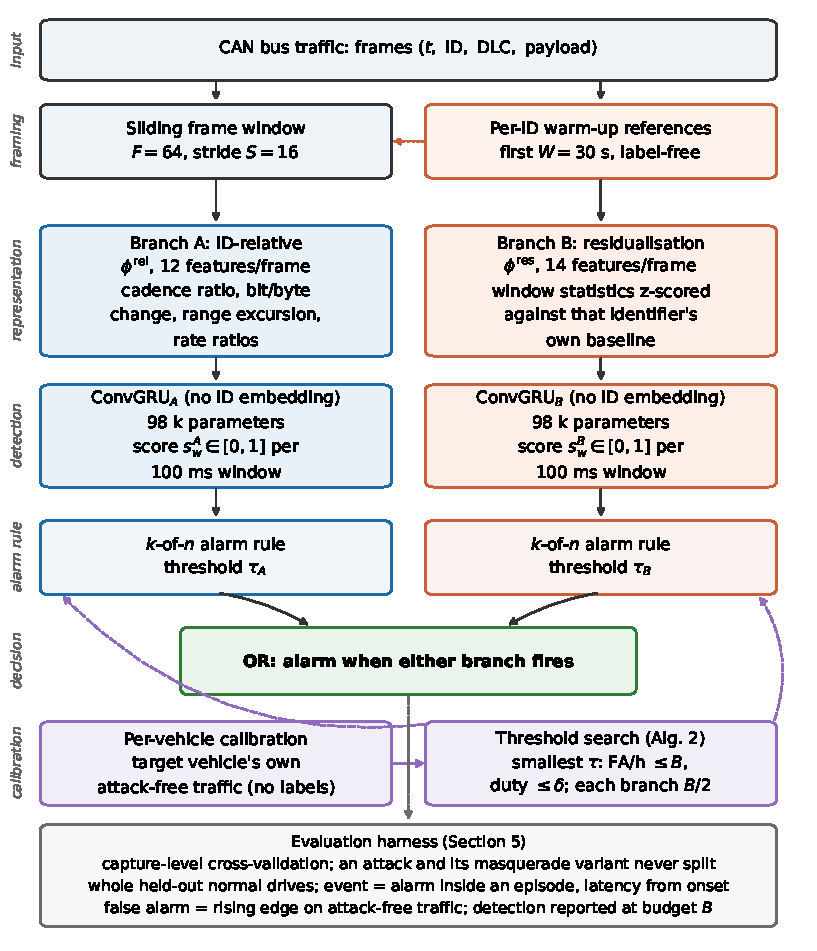
\includegraphics[width=\textwidth]{figs/architecture.pdf}
\caption{Architecture of the proposed detector and of the evaluation harness that surrounds it.
Frames arriving on the bus are cut into sliding windows of $F$ consecutive frames. Per-identifier
reference statistics are estimated once from a \SI{30}{\second} warm-up prefix of the capture
(orange, label-free). Two identifier-agnostic representations are computed from the same frames:
branch A (blue) describes each frame by ratios against its own identifier's references, branch B
(orange) by window statistics z-scored against the same references. Each branch feeds an
embedding-free ConvGRU that emits one score per \SI{100}{\milli\second} window; each score stream is
converted into alarms by a $k$-of-$n$ rule whose threshold is calibrated on the target vehicle's own
attack-free traffic to satisfy half of the false-alarm budget (purple). An alarm is raised when
either branch fires. The grey band lists the evaluation rules of Section~\ref{sec:math}, which apply
to every detector we compare, not only to ours.}
\label{fig:arch}
\end{figure*}

Figure~\ref{fig:arch} shows the complete pipeline, which has four stages and one calibration path.

\paragraph{Stage 1: framing and references.} Bus traffic is a stream of frames
$(t_i,\mathrm{ID}_i,\mathrm{DLC}_i,\mathbf{b}_i)$. The stream is cut into sliding windows of
$F=64$ consecutive frames with stride $16$, and independently into fixed \SI{100}{\milli\second}
time windows that carry the labels and the alarm logic. From the first $W=\SI{30}{\second}$ of each
capture the system estimates, for every arbitration identifier observed, a small set of reference
statistics: median inter-arrival time, frame rate, per-byte minimum and maximum, modal DLC, and the
mean and standard deviation of the window statistics used by branch B. These references require no
labels, which is what makes per-vehicle commissioning practical.

\paragraph{Stage 2: two identifier-agnostic representations.} Branch A computes twelve per-frame
features that are all ratios or deviations with respect to the frame's own identifier: cadence ratio
against the reference inter-arrival time, bit- and byte-change fractions against the previous frame
of that identifier, excursion beyond the reference byte range, per-identifier and bus-wide rate
ratios, and a DLC-change indicator. Branch B computes fourteen window statistics per identifier --
temporal, protocol and payload -- and z-scores them against the same references, following the
residualisation idea of \citet{hegde2026residualization}. In both branches the identifier is used
only to group frames \emph{within} a capture; it never enters the model as a learned embedding and
no identifier vocabulary is carried between vehicles. This is the property that survives a change of
vehicle.

\paragraph{Stage 3: detectors.} Each branch feeds a small convolutional--recurrent network
(ConvGRU) of 98\,k parameters: two 1-D convolutions over the frame axis, a bidirectional GRU, and a
linear head producing one score per window. The two branches are otherwise identical and are trained
independently on the source vehicle's labelled attacks.

\paragraph{Stage 4: alarm logic.} Each score stream passes through a $k$-of-$n$ rule: the branch is
in alarm when at least $k$ of the last $n$ window scores exceed its threshold. The system raises an
alarm when either branch is in alarm. Because a union of two detectors doubles the opportunity to
fire, each branch is calibrated to half of the total false-alarm budget, which keeps the comparison
against single branches fair.

\paragraph{Calibration path.} Thresholds are not transferred from the source vehicle. At
commissioning, attack-free traffic from the target vehicle is scored, and each branch receives the
smallest threshold that satisfies both the false-alarm budget and the duty cap
(Algorithm~\ref{alg:calib}). No labelled attacks from the target vehicle are required.

\section{Mathematical modelling}
\label{sec:math}

\subsection{Notation and windows}

Table~\ref{tab:notation} lists the notation. Let a capture be a finite frame sequence
$\mathcal{F}=\{(t_i,\mathrm{ID}_i,\mathrm{DLC}_i,\mathbf{b}_i)\}_{i=1}^{N}$ with $t_i$ increasing,
$\mathrm{ID}_i\in\mathcal{I}$ the arbitration identifier, and $\mathbf{b}_i\in\{0,\dots,255\}^8$ the
payload. Fix a window length $\Delta=\SI{100}{\milli\second}$ and let
$w(i)=\lfloor (t_i-t_1)/\Delta\rfloor$ be the window index of frame $i$; window $w$ contains
$\mathcal{W}_w=\{i: w(i)=w\}$ and there are $T$ windows.

\begin{table}[t]
\centering
\caption{Notation.}
\label{tab:notation}
\small
\begin{tabular}{ll}
\toprule
Symbol & Meaning\\
\midrule
$\mathcal{F}$, $N$ & frame sequence of a capture and its length\\
$\Delta$, $T$, $w$ & window length (\SI{100}{\milli\second}), number of windows, window index\\
$F$, $S$ & frame-window length ($64$) and stride ($16$)\\
$W$ & warm-up horizon for per-identifier references (\SI{30}{\second})\\
$\mathcal{I}$, $\mu_{\mathrm{ID}}$ & identifier alphabet of a capture; reference statistics of identifier $\mathrm{ID}$\\
$\phirel,\phires$ & identifier-agnostic representations (12 and 14 features per frame)\\
$s_w\in[0,1]$ & detector score of window $w$\\
$y_w\in\{0,1\}$ & window label: an injected frame is present (after gap filling)\\
$\mathcal{E}=\{(o_e,c_e)\}$ & attack episodes, onset and end window\\
$a_w(\tau;k,n)$ & alarm indicator of the $k$-of-$n$ rule at threshold $\tau$\\
$B$, $\delta$ & false-alarm budget (per hour) and alarm duty cap\\
$D(\tau)$, $\FA(\tau)$, $\rho(\tau)$ & events detected, false alarms per hour, alarm duty\\
$\ell_e(\tau)$ & detection latency of episode $e$\\
\bottomrule
\end{tabular}
\end{table}

\subsection{Identifier-agnostic representations}

Let $p(i)$ be the index of the previous frame with the same identifier. For identifier $u\in
\mathcal{I}$ let $\mathcal{W}^u=\{i:\mathrm{ID}_i=u\}$ and let the warm-up set be
$\mathcal{W}^u_W=\{i\in\mathcal{W}^u: t_i-t_1\le W\}$. The references are
\begin{align}
m_u &= \operatorname{median}\{\,t_i-t_{p(i)} : i\in\mathcal{W}^u_W\,\}, &
r_u &= \frac{|\mathcal{W}^u_W|}{\max(t_{\max}-t_1,1)}\,\Delta, \label{eq:refs}\\
\underline{b}_{u,c} &= \min_{i\in\mathcal{W}^u_W} b_{i,c}, &
\overline{b}_{u,c} &= \max_{i\in\mathcal{W}^u_W} b_{i,c}, \qquad c=1,\dots,8 . \nonumber
\end{align}
Branch A maps frame $i$ with $u=\mathrm{ID}_i$ to $\phirel(i)\in\mathbb{R}^{12}$, whose components
include the cadence ratio and the range excursion
\begin{equation}
\phirel_1(i)=\frac{t_i-t_{p(i)}}{m_u},
\qquad
\phirel_9(i)=\max_{c}\;\frac{\max\!\big(\underline{b}_{u,c}-b_{i,c},\; b_{i,c}-\overline{b}_{u,c}\big)}
{\max(\overline{b}_{u,c}-\underline{b}_{u,c},1)},
\label{eq:rel}
\end{equation}
together with bit- and byte-change fractions with respect to frame $p(i)$, the
fraction of bytes below and above the reference range, per-identifier and bus-wide rate ratios, and a
DLC-change indicator. Branch B first forms, for each window $w$ and identifier $u$, a vector
$x_{w,u}\in\mathbb{R}^{14}$ of temporal, protocol and payload statistics, then residualises it,
\begin{equation}
\phires_{w,u} \;=\; \operatorname{clip}\!\left(\frac{x_{w,u}-\mu_u}{\sigma_u},\,-20,\,20\right),
\qquad
(\mu_u,\sigma_u)=\big(\operatorname{mean},\operatorname{sd}\big)\{x_{w,u}: w\Delta\le W\},
\label{eq:res}
\end{equation}
and assigns to frame $i$ the vector of its own identifier and window. Both maps are invariant to a
relabelling of $\mathcal{I}$: they never use the numeric value or the learned embedding of an
identifier, only statistics computed within its own stream. This is the formal sense in which the
representation is identifier-agnostic, and it is the property that Section~\ref{sec:transfer} shows
to be necessary for cross-vehicle transfer.

\subsection{Labels, episodes and alarms}

Window $w$ is attacked, $y_w=1$, if it contains at least one injected frame; because sparse
injections leave gaps, we close gaps shorter than \SI{1}{\second} so that one injection interval
yields one episode. Episodes are the maximal runs of $y=1$,
$\mathcal{E}=\{(o_e,c_e)\}_{e=1}^{E}$, with onset $o_e$ and end $c_e$.

Given scores $s_w$ and threshold $\tau$, the $k$-of-$n$ alarm indicator is
\begin{equation}
a_w(\tau;k,n) \;=\; \mathbb{1}\!\left[\;\sum_{j=\max(1,w-n+1)}^{w}\mathbb{1}[s_j\ge\tau]\;\ge\;k\;\right].
\label{eq:kofn}
\end{equation}
An episode is \emph{detected} if the rule fires inside it, and its latency is the time from onset to
the first such alarm,
\begin{equation}
d_e(\tau)=\mathbb{1}\!\left[\exists\,w\in[o_e,c_e]: a_w(\tau)=1\right],
\qquad
\ell_e(\tau)=\Delta\cdot\min\{\,w-o_e:\; w\in[o_e,c_e],\,a_w(\tau)=1\,\}.
\label{eq:detect}
\end{equation}
A \emph{false alarm} is a rising edge on attack-free traffic. Writing $\mathcal{C}$ for the set of
attack-free windows (all windows of an attack-free capture, and the pre-onset windows of an attack
capture) and $H=\Delta|\mathcal{C}|/3600$ for their duration in hours,
\begin{equation}
\FA(\tau)=\frac{1}{H}\sum_{w\in\mathcal{C}}\mathbb{1}\!\left[a_w(\tau)=1 \wedge a_{w-1}(\tau)=0\right],
\qquad
\rho(\tau)=\frac{1}{|\mathcal{C}|}\sum_{w\in\mathcal{C}} a_w(\tau).
\label{eq:fa}
\end{equation}
The duty $\rho$ is what prevents a degenerate solution: a threshold so low that the alarm never
clears produces exactly one rising edge per capture and therefore an arbitrarily small $\FA$, while
being useless. We require $\rho\le\delta$ with $\delta=0.02$.

\subsection{Budget-constrained detection}

The quantity we report throughout is the number of events detected at a false-alarm budget,
\begin{equation}
D^\star(B) \;=\; \max_{\tau\,\in\,\mathcal{T}}\; \sum_{e=1}^{E} d_e(\tau)
\quad\text{subject to}\quad \FA(\tau)\le B,\;\; \rho(\tau)\le\delta ,
\label{eq:objective}
\end{equation}
where $\mathcal{T}$ is a grid of candidate thresholds. Two properties of
\eqref{eq:objective} matter in practice. First, $D^\star$ is not monotone in the grid resolution:
a coarse $\mathcal{T}$ can miss the feasible region entirely, which is the first evaluation trap of
Section~\ref{sec:traps}; we use $|\mathcal{T}|=200$ quantiles of the observed scores. Second, when
the threshold must be chosen without access to test data -- the deployment case -- it is calibrated
on separate attack-free traffic $\mathcal{C}_{\mathrm{cal}}$, and the achieved $\FA$ on test data is
reported alongside, so that a failure of threshold transfer is visible rather than hidden.

For the paired detector, branch scores $s^A,s^B$ with thresholds $\tau_A,\tau_B$ produce the union
alarm
\begin{equation}
a^{A\vee B}_w \;=\; a^A_w(\tau_A;k,n)\;\vee\;a^B_w(\tau_B;k,n),
\label{eq:union}
\end{equation}
and each branch is calibrated to budget $B/2$ so that, in the worst case of disjoint false alarms,
the union still satisfies $B$.

\section{Proposed algorithms}
\label{sec:algo}

Algorithm~\ref{alg:features} states the label-free construction of per-identifier references and of
the two representations; it is executed once per capture and is the only step that touches
identifiers. Its cost is linear in the number of frames, $O(N)$ time and $O(|\mathcal{I}|)$ memory
for the references, so it is suitable for streaming implementation on a gateway ECU. The warm-up
requirement is the practical price: the first $W$ seconds after ignition are used to estimate
references and are excluded from evaluation.

\begin{algorithm}[t]
\caption{Identifier-agnostic feature construction (per capture, no labels)}
\label{alg:features}
\begin{algorithmic}[1]
\Require frames $\mathcal{F}$, warm-up $W$, window length $\Delta$
\Ensure per-frame representations $\phirel$, $\phires$
\ForAll{identifiers $u$ observed in the warm-up prefix $t_i-t_1\le W$}
  \State compute references $m_u$, $r_u$, $\underline{b}_{u,\cdot}$, $\overline{b}_{u,\cdot}$, modal DLC \Comment{Eq.~\eqref{eq:refs}}
  \State compute window statistics $x_{w,u}$ for warm-up windows and their $(\mu_u,\sigma_u)$
\EndFor
\ForAll{frames $i$ with $t_i-t_1 > W$}
  \State $u\gets \mathrm{ID}_i$; $p\gets$ index of previous frame of identifier $u$
  \State $\phirel(i)\gets$ cadence, change, excursion and rate ratios w.r.t. $(m_u,r_u,\underline{b}_u,\overline{b}_u)$ \Comment{Eq.~\eqref{eq:rel}}
  \State $\phires(i)\gets \operatorname{clip}\big((x_{w(i),u}-\mu_u)/\sigma_u,-20,20\big)$ \Comment{Eq.~\eqref{eq:res}}
\EndFor
\State \Return $\phirel,\phires$
\end{algorithmic}
\end{algorithm}

Algorithm~\ref{alg:calib} is the calibration procedure. It searches the smallest feasible threshold,
which is the most sensitive one that respects both constraints of \eqref{eq:objective}; the search
is over a grid of score quantiles and costs $O(|\mathcal{T}|\,|\mathcal{C}_{\mathrm{cal}}|)$. The
duty test on line~6 is what distinguishes it from the usual practice of maximising $F_1$ on a
validation set, and the fact that it uses only attack-free traffic is what makes per-vehicle
commissioning possible without labelled attacks.

\begin{algorithm}[t]
\caption{Per-vehicle threshold calibration under a false-alarm budget}
\label{alg:calib}
\begin{algorithmic}[1]
\Require attack-free calibration scores $\{s_w\}_{w\in\mathcal{C}_{\mathrm{cal}}}$, budget $B$,
duty cap $\delta$, rule $(k,n)$
\Ensure threshold $\tau^\star$
\State $\mathcal{T}\gets$ 200 quantiles of $\{s_w\}$, sorted ascending
\ForAll{$\tau\in\mathcal{T}$}
  \State $a_w \gets k$-of-$n$ rule applied to $\{s_w\ge\tau\}$ \Comment{Eq.~\eqref{eq:kofn}}
  \State $\FA \gets$ rising edges of $a$ per hour; $\rho \gets$ mean of $a$ \Comment{Eq.~\eqref{eq:fa}}
  \If{$\FA \le B$ \textbf{and} $\rho \le \delta$}
     \State \Return $\tau^\star \gets \tau$ \Comment{most sensitive feasible threshold}
  \EndIf
\EndFor
\State \Return $\tau^\star \gets \max\mathcal{T} + \epsilon$ \Comment{infeasible: report as such}
\end{algorithmic}
\end{algorithm}

Algorithm~\ref{alg:detect} is the runtime procedure of the paired detector. Each branch is evaluated
independently and the alarms are combined by disjunction, with each branch calibrated to half the
budget. The per-window cost is two ConvGRU evaluations plus $O(1)$ alarm bookkeeping;
Section~\ref{sec:cost} measures it.

\begin{algorithm}[t]
\caption{Paired identifier-agnostic detection at run time}
\label{alg:detect}
\begin{algorithmic}[1]
\Require frame stream, models $g_A,g_B$, thresholds $\tau_A,\tau_B$ from Algorithm~\ref{alg:calib}
with budget $B/2$ each, rule $(k,n)$
\Ensure alarm events
\State collect the warm-up prefix and build references \Comment{Algorithm~\ref{alg:features}}
\ForAll{arriving frame windows $(i-F,\dots,i)$ with stride $S$}
  \State $s^A \gets g_A(\phirel(i-F{:}i))$; \quad $s^B \gets g_B(\phires(i-F{:}i))$
  \State assign $s^A,s^B$ to the \SI{100}{\milli\second} window containing $t_i$ (maximum if several)
  \State $a^A \gets k$-of-$n(s^A\ge\tau_A)$; \quad $a^B \gets k$-of-$n(s^B\ge\tau_B)$
  \If{$a^A \vee a^B$ and no alarm was active in the previous window}
     \State emit alarm event with timestamp $t_i$ \Comment{Eq.~\eqref{eq:union}}
  \EndIf
\EndFor
\end{algorithmic}
\end{algorithm}

\section{Datasets}
\label{sec:data}

Table~\ref{tab:datasets} summarises the three corpora as we use them, after preprocessing.

\begin{table}[t]
\centering
\caption{Corpora as used in this study, after preprocessing. ``Normal'' is the attack-free traffic
available for calibration and false-alarm measurement.}
\label{tab:datasets}
\small
\begin{tabular}{llrrrl}
\toprule
Corpus & Role & Vehicles & Events & Normal & Attack types\\
\midrule
Car-Hacking \citep{song2020dcnn} & benchmark critique & 1 & $4\times300$ & \SI{481.6}{\second} &
DoS, fuzzy, gear, RPM\\
ROAD \citep{verma2024road} & main detection study & 1 & 29 & \SI{72}{\minute} &
fuzzing, targeted injection, masquerade\\
can-train-and-test \citep{lampe2023cantt} & cross-vehicle study & 4 & 44 (+26 masq.) & \SI{22}{\minute}/pair &
DoS, spoofing, interval, standstill, masquerade\\
\bottomrule
\end{tabular}
\end{table}

\paragraph{Car-Hacking.} Four attack captures and one attack-free capture from a single vehicle.
Parsing the raw logs reveals two artefacts that affect any user of this corpus. First, each attack
file contains exactly 300 injection episodes whose inter-episode gaps are \SI{3.0}{\second} with a
coefficient of variation of 0.001--0.003 (Fig.~\ref{fig:carhacking}a); the schedule is therefore
almost perfectly periodic. Second, the same \SI{481.6}{\second} attack-free recording
(891{,}068 byte-identical frames) is appended to all four attack files, and
\texttt{Fuzzy\_dataset.csv} additionally contains two recording sessions separated by a
\SI{2540}{\second} silence. Without de-duplication the attack-free traffic is counted four times;
without splitting at the silence, a chronological split places every attack in the training portion
and none in validation or test. We do both.

\paragraph{ROAD.} We use the nine dynamometer ambient captures (\SI{72}{\minute} of attack-free
driving) and every attack capture with a labelled injection interval: 15 physically verified
injection events, 14 of which also exist as masquerade variants in which conflicting legitimate
frames were removed, giving 29 attack events. Frame labels are reconstructed from the published
metadata -- injection interval, target identifier, and a byte pattern with wildcards. As a
consistency check, in non-masquerade captures the target identifier carries exactly twice as many
frames inside the interval as there are injected frames (injected plus displaced legitimate), and in
the masquerade variants the two counts coincide; our reconstruction reproduces this for all
captures, and every reconstructed episode begins within one window of the published onset. The four
accelerator captures carry no injected frames and are excluded.

\paragraph{can-train-and-test.} Four sub-datasets, each nominating a known and an unknown vehicle:
Impala$\rightarrow$Silverado, Traverse$\rightarrow$Forester, Silverado$\rightarrow$Forester and
Forester$\rightarrow$Traverse, the last three crossing manufacturers. We use the attack-free training
subset, the attack training subset, the known-vehicle and unknown-vehicle test subsets and the
masquerade subset. The target vehicles have up to 98 arbitration identifiers against 52 for the
source, which is one reason identifier-embedding models fail to transfer.

\section{Experimental setup}
\label{sec:setup}

\paragraph{Protocol parameters.} $\Delta=\SI{100}{\milli\second}$, $F=64$ frames, stride $S=16$,
warm-up $W=\SI{30}{\second}$, gap filling \SI{1}{\second}, duty cap $\delta=0.02$, alarm rules
$(k,n)\in\{(1,1),(2,3),(3,5)\}$ with $(3,5)$ as default, budgets
$B\in\{5,10,30,60\}$ \si{\per\hour}, threshold grid $|\mathcal{T}|=200$.

\paragraph{Models.} The ConvGRU has two 1-D convolutions (64 channels, kernel 5, the second
strided), a bidirectional GRU (64 units) and a two-layer head; with an identifier embedding of 32
dimensions it has 98\,k parameters, and the embedding-free variants used in
Section~\ref{sec:transfer} are of the same size. It is trained for 15 epochs of 600 steps, batch
512, AdamW at $10^{-3}$, with positive class weight 5. The spatio-temporal graph model (referred to
as the graph-attention model) applies two dense graph-attention layers with four heads over the
identifier graph of each window, a four-layer Transformer encoder over a 20-window history,
per-horizon heads and Monte-Carlo dropout; $d_{\mathrm{model}}=128$, 1.05\,M parameters, AdamW at
$3\times10^{-4}$, 25 epochs with early stopping (patience 6), batch 32. The window GBDT is a
histogram gradient-boosting classifier (300 iterations, balanced class weights) over all
identifiers' features in the current window. The two unsupervised detectors are exceedance tests
against per-identifier normal ranges, one on frame counts and one on per-(identifier, byte) payload
novelty.

\paragraph{Cross-validation.} On ROAD, fold $f\in\{0,1,2\}$ tests attack instance $f{+}1$, validates
on the next instance and trains on the remainder; an attack and its masquerade variant always share
a split. Ambient captures are assigned whole to training, calibration or test, rotating with the
fold. On can-train-and-test we use the corpus's own known/unknown vehicle split.

\paragraph{Seeds and statistics.} Unless stated otherwise, learned models are run with five seeds on
ROAD and three on can-train-and-test; we report mean $\pm$ standard deviation. Model pairs are
compared with the Mann--Whitney $U$ test over seeds and, for detected-event sets at a common budget,
with an exact McNemar test.

\paragraph{Hardware.} Training and inference use one NVIDIA RTX 5060 Laptop GPU (8\,GB), 16\,GB RAM,
PyTorch 2.11 with CUDA 12.8. Cost measurements in Section~\ref{sec:cost} use a single CPU thread at
batch size 1.

\section{What the standard benchmarks measure}
\label{sec:benchmarks}

\subsection{Car-Hacking rewards learning the schedule}

\begin{figure}[t]
\centering
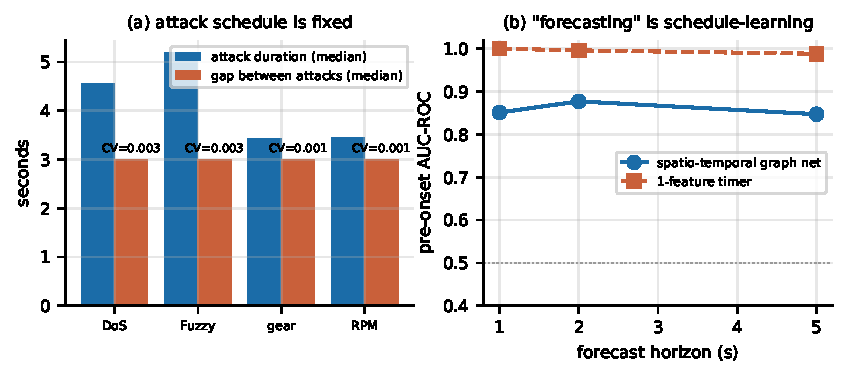
\includegraphics[width=\linewidth]{figs/carhacking_schedule.pdf}
\caption{Car-Hacking. (a) Median attack duration and median gap between consecutive attacks for the
four attack files; the gap is \SI{3.0}{\second} in every file, with coefficient of variation between
0.001 and 0.003. (b) Pre-onset AUC-ROC -- computed only on windows in which no attack is yet in
progress -- for a spatio-temporal graph network and for a logistic model whose only feature is the
time since the last attack. The timer is at or above the network at every horizon, so what is being
measured is the injection schedule.}
\label{fig:carhacking}
\end{figure}

Figure~\ref{fig:carhacking}a shows why the corpus cannot support claims about anticipating attacks.
Its attacks follow a timetable, so the optimal predictor of the next onset is a clock.
Figure~\ref{fig:carhacking}b makes this concrete on the fuzzy capture: restricted to pre-onset
windows, a one-feature timer attains AUC 1.000, 0.996 and 0.988 at horizons of 1, 2 and
\SI{5}{\second}, against 0.851, 0.877 and 0.847 for the graph network with Monte-Carlo dropout.
Pooling all four attack files the ordering persists at \SI{1}{\second} (0.980 against 0.901). We
therefore regard published look-ahead results on this corpus as unsupported unless they report a
timing-only baseline.

Detection on the same corpus is saturated: the graph model reaches $F_1=0.9997$ at AUC 1.000 when
asked whether the current window contains an attack, matching the near-perfect numbers common in the
literature \citep{song2020dcnn,lo2022hydlids,rai2025securing} and leaving no headroom in which a new
method could demonstrate an advantage. This is consistent with the redundancy analysis of
\citet{le2026cicio} on a different corpus.

\subsection{On ROAD, architectural complexity does not pay}

\begin{figure}[t]
\centering
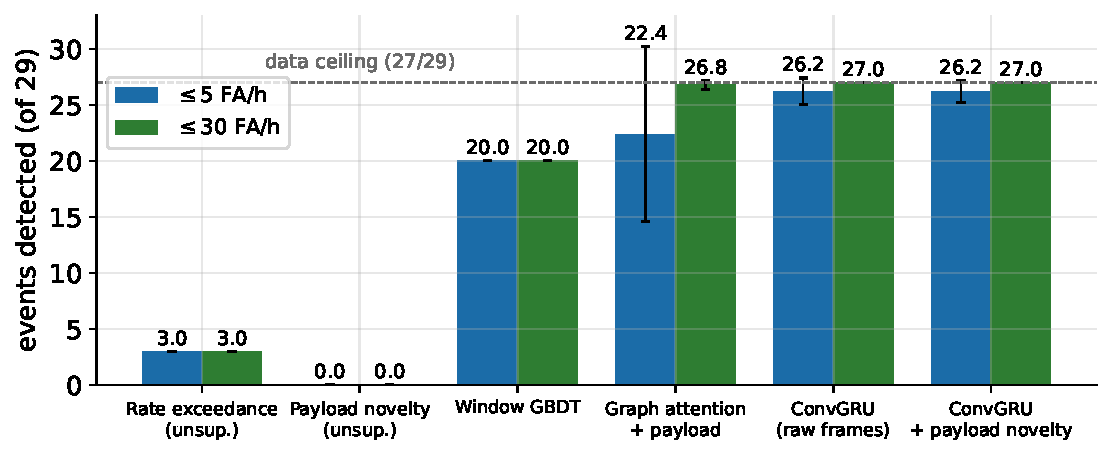
\includegraphics[width=\linewidth]{figs/model_comparison.pdf}
\caption{ROAD: events detected of 29 at two false-alarm budgets, 3-of-5 alarm rule, alarm duty
$\le2\%$. Learned models use five seeds (error bars are one standard deviation); the unsupervised
detectors and the GBDT are deterministic given the fold. The dashed line marks the ceiling of 27
events that no configuration exceeds.}
\label{fig:comparison}
\end{figure}

\begin{table}[t]
\centering
\caption{ROAD, 3-fold capture-level cross-validation, 29 attack events, \SI{1.2}{\hour} of held-out
attack-free driving, 3-of-5 alarm rule. Events detected (mean $\pm$ s.d. over seeds).}
\label{tab:road}
\begin{tabular}{lrrr}
\toprule
Model & Params & $\leq$\SI{5}{\per\hour} & $\leq$\SI{30}{\per\hour}\\
\midrule
Rate exceedance (unsupervised)     & --      & 3/29 & 3/29\\
Payload novelty (unsupervised)     & --      & 0/29 & 0/29\\
Window GBDT (no graph, no history) & --      & 20/29 & 20/29\\
Graph attention + payload novelty  & 1.05\,M & $22.4\pm7.8$ & $26.8\pm0.4$\\
ConvGRU on raw frames              & 98\,k   & $\mathbf{26.2\pm1.2}$ & $\mathbf{27.0\pm0.0}$\\
ConvGRU + payload novelty          & 98\,k   & $26.2\pm1.0$ & $\mathbf{27.0\pm0.0}$\\
\bottomrule
\end{tabular}
\end{table}

Table~\ref{tab:road} and Figure~\ref{fig:comparison} report the comparison. The three learned models
are statistically indistinguishable: ConvGRU against ConvGRU with payload novelty gives $p=1.000$
with identical detected-event sets under McNemar, and either against the graph model gives $p=0.81$
at \SI{5}{\per\hour} and $p=0.42$ at \SI{30}{\per\hour} under Mann--Whitney. All three stop at 27 of
29 events. The two events that no model detects are the engine-coolant-temperature injection and its
masquerade variant, which deliver 43 frames over \SI{4}{\second}; the ceiling is therefore a property
of the data, not of the models. The 98\,k-parameter model is ten times smaller, twenty-nine times
faster per inference (Section~\ref{sec:cost}) and considerably more stable across seeds than the
1.05\,M-parameter one.

Figure~\ref{fig:curves} shows the full trade-off from which those two operating points are taken.
The unsupervised detectors are unusable at any budget, the GBDT saturates at 20 events, and the
learned sequence models converge to the ceiling once the budget exceeds roughly 20 alarms per hour.

\begin{figure}[t]
\centering
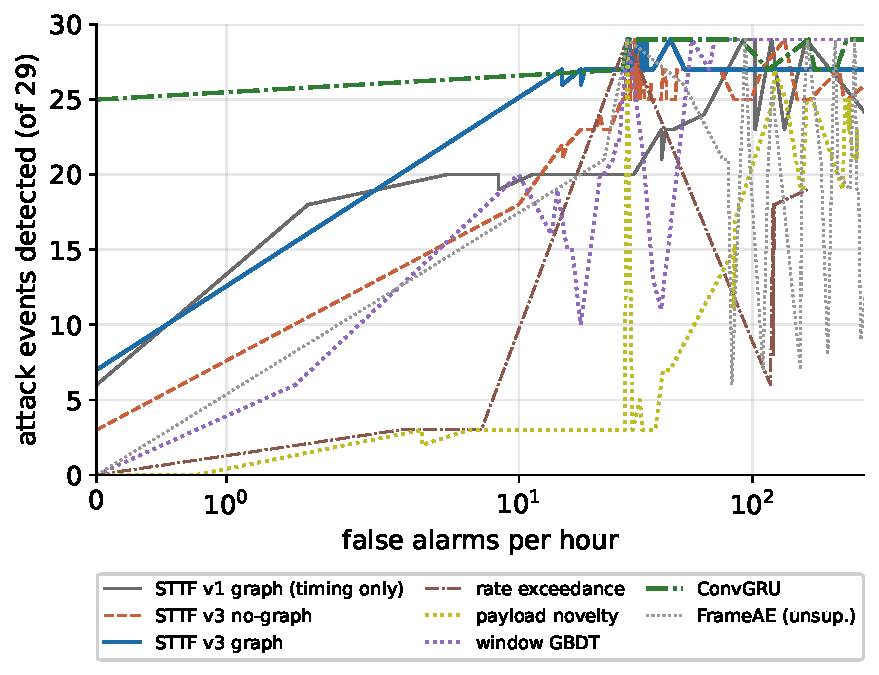
\includegraphics[width=0.74\linewidth]{figs/road_event_curves.pdf}
\caption{ROAD: attack events detected against false alarms per hour of held-out attack-free driving,
sweeping the threshold (3-of-5 rule, duty $\le2\%$, folds pooled, seed 0). Curves that rise only at
high alarm rates are unusable in a vehicle regardless of their AUC.}
\label{fig:curves}
\end{figure}

\subsection{A detectability hierarchy}

\begin{figure}[t]
\centering
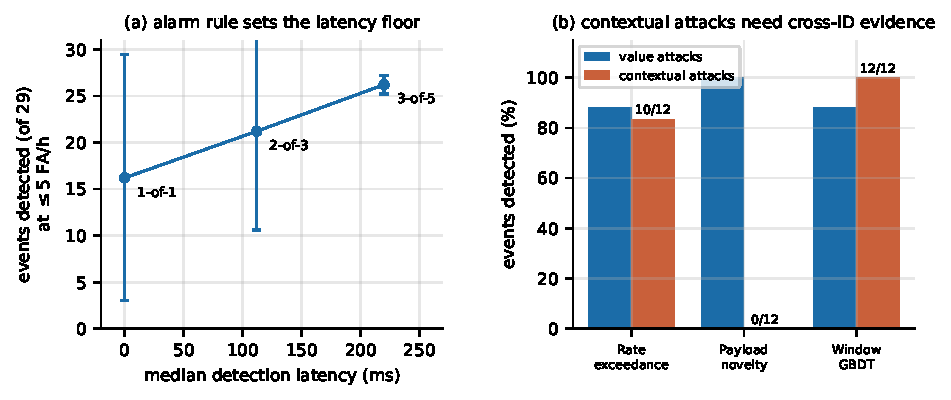
\includegraphics[width=\linewidth]{figs/latency_tiers.pdf}
\caption{(a) Events detected against median detection latency for three alarm rules
(ConvGRU + payload novelty, five seeds, $\leq$\SI{5}{\per\hour}); the rule, not the model, sets the
latency floor, and the fastest rule is also the least stable. (b) Detection by attack tier: the
per-(identifier, byte) novelty detector finds every value attack and no contextual attack, while a
model that sees all identifiers jointly finds all contextual attacks.}
\label{fig:latency}
\end{figure}

Attacks fall into three tiers, and the tier decides what evidence is required.
Figure~\ref{fig:latency}b quantifies the distinction on ROAD. \emph{Rate} attacks change an
identifier's frame rate and are found by a frame-count exceedance test (15 of 17 value attacks, 10 of
12 contextual). \emph{Value} attacks write byte values the identifier never normally carries: the
per-(identifier, byte) novelty test finds 17 of 17. \emph{Contextual} attacks write an ordinary value
that is wrong only given other identifiers -- ROAD's reverse-light attacks set the light state while
the vehicle is not in reverse -- and the same novelty test finds 0 of 12, while the GBDT, which sees
all identifiers jointly, finds 12 of 12. Cross-identifier evidence is therefore necessary for the
third tier, but a graph neural network is not: a flat model over all identifiers suffices.

\subsection{Latency is set by the alarm rule}

Figure~\ref{fig:latency}a and Table~\ref{tab:latency} separate model latency from rule latency. A
$k$-of-$n$ rule cannot fire before $k$ windows have exceeded the threshold, so the rule imposes a
floor of $(k-1)\Delta$. The unsmoothed 1-of-1 rule detects inside the onset window -- a median
latency of \SI{0}{\milli\second}, i.e. below \SI{100}{\milli\second} -- but has no feasible threshold
for two of five seeds, whereas the stable 3-of-5 rule costs \SI{220}{\milli\second}. Reporting a
sub-\SI{100}{\milli\second} latency therefore requires stating the alarm rule and its stability;
otherwise the number is not comparable between papers.

\begin{table}[t]
\centering
\caption{Latency and stability by alarm rule. ConvGRU with payload novelty at $\leq$\SI{5}{\per\hour},
five seeds, ROAD.}
\label{tab:latency}
\begin{tabular}{lrrl}
\toprule
Rule & Events detected & Median latency & Note\\
\midrule
1-of-1 & $16.2\pm13.2$ & \SI{0}{\milli\second} & no feasible threshold for 2/5 seeds\\
2-of-3 & $21.2\pm10.6$ & \SI{112}{\milli\second} & 1/5 seeds infeasible\\
3-of-5 & $\mathbf{26.2\pm1.0}$ & \SI{220}{\milli\second} & stable\\
\bottomrule
\end{tabular}
\end{table}

\section{Five evaluation traps}
\label{sec:traps}

Table~\ref{tab:traps} lists five choices that, applied alone to the same code and data, reverse the
ranking of the models in Table~\ref{tab:road}. We encountered each of them in the course of this
study, in the order shown, and each initially produced a confident conclusion that a stricter
protocol subsequently removed.

\begin{table}[t]
\centering
\caption{Five evaluation choices, each sufficient on its own to reverse model rankings. ``Permissive''
is the choice that produced the wrong conclusion; ``strict'' is the setting used in this paper.}
\label{tab:traps}
\small
\begin{tabular}{p{0.21\linewidth}p{0.36\linewidth}p{0.36\linewidth}}
\toprule
Choice & Permissive setting and its conclusion & Strict setting and the true result\\
\midrule
Threshold-grid resolution & 60 candidate thresholds: payload-novelty features add $+4.2$ events,
$p=0.029$ & 200 candidates: $p=1.000$, identical detected-event sets\\
Seed count & 3 seeds: graph attention adds 11 events over its ablation & 5 seeds: $p=0.81$;
single-seed scores range from 7 to 27 events\\
Duty cap during threshold selection & absent: ``29/29 events at \SI{29}{\per\hour}'' from an alarm
that never clears & present: the alarm must clear; 27/29 at \SI{28}{\per\hour}\\
Duty cap on reported metrics & absent: 8/8 events on an unseen vehicle & present: the alarm is
active 99.9\% of the time; 0/8 events\\
Composition of held-out normal traffic & time slices of the drives used for testing: a
\SI{60}{\per\hour} budget appears to transfer & whole held-out drives: the same budget yields
1244--\SI{2866}{\per\hour} on unseen drives\\
\bottomrule
\end{tabular}
\end{table}

\begin{figure}[t]
\centering
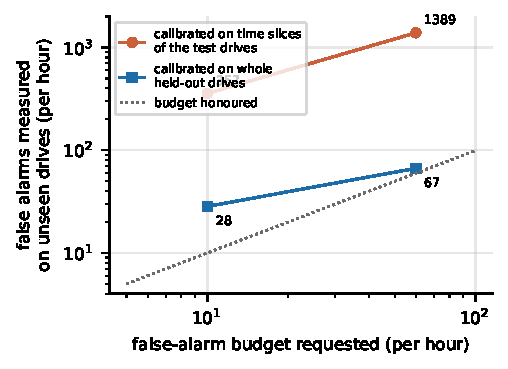
\includegraphics[width=0.56\linewidth]{figs/threshold_transfer.pdf}
\caption{The fifth trap made visible. A threshold is calibrated to a requested false-alarm budget
(horizontal axis) and the rate it actually achieves on unseen normal driving is measured (vertical
axis); the dotted line is the budget being honoured. Calibrating on time slices of the same drives
used for testing (orange) overshoots by one to two orders of magnitude, because the calibration and
test traffic are statistically the same drive. Calibrating on whole held-out drives (blue) keeps the
achieved rate within a small factor of the request. Graph-attention model, 3-of-5 rule.}
\label{fig:transfer}
\end{figure}

The first two are statistical: a coarse threshold grid can miss the feasible region of
\eqref{eq:objective} entirely, and three seeds cannot resolve a difference when the seed standard
deviation reaches eight events. The third and fourth concern the degenerate solution that
\eqref{eq:fa} admits without a duty constraint; the fourth is particularly insidious because it
appears only when the detector is applied to data unlike its training data, which is exactly the
cross-vehicle case. The fifth is a data-composition choice that silently converts a calibration
experiment into an interpolation experiment, and Figure~\ref{fig:transfer} shows its magnitude: a
budget of \SI{10}{\per\hour} calibrated on time slices of the test drives yields
\SI{357}{\per\hour} in practice, whereas the same budget calibrated on whole held-out drives yields
\SI{28}{\per\hour}. None of the five traps is expensive to avoid; all five are invisible in a table
of $F_1$ scores.

\section{Cross-vehicle transfer}
\label{sec:transfer}

\subsection{Identifier-embedding detectors transfer to nothing}

\begin{figure}[t]
\centering
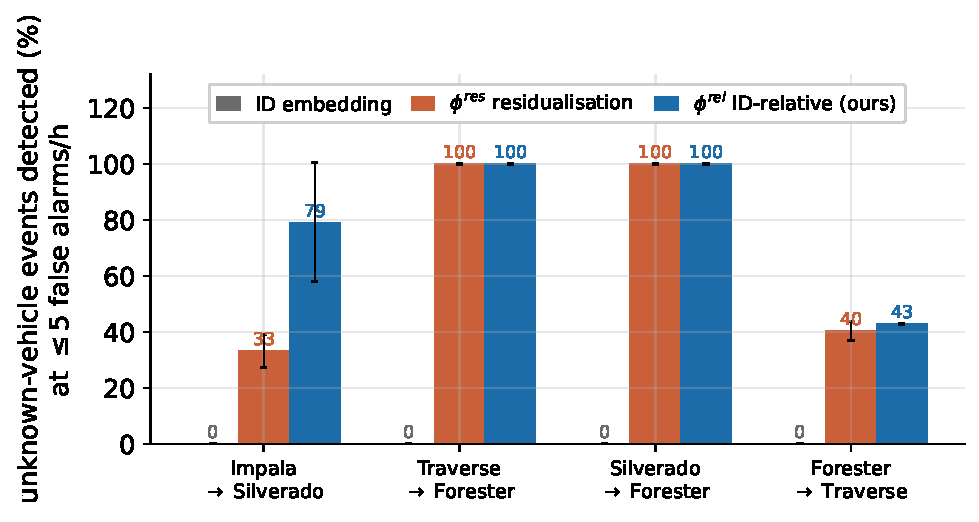
\includegraphics[width=0.74\linewidth]{figs/cross_vehicle.pdf}
\caption{Unknown-vehicle events detected at $\leq$\SI{5}{\per\hour} false alarms, thresholds
calibrated on the target vehicle's own attack-free traffic without labels, three seeds. The
identifier-embedding detector scores zero on every pair; both identifier-agnostic representations
transfer.}
\label{fig:cross}
\end{figure}

Trained on one vehicle of a can-train-and-test pair and evaluated on the other, the standard
identifier-embedding detector detects 0 of 44 events at a valid operating point
(Fig.~\ref{fig:cross}, grey). The unconstrained numbers look excellent -- with the source vehicle's
threshold it flags 8 of 8 events on the first pair -- but its alarm is then active 99.9\% of the
time, and once the threshold must satisfy a budget on the target vehicle's own attack-free traffic,
detection falls to zero. Removing the payload features changes nothing, so this is not an artefact of
one feature set: the learned identifier embeddings and traffic patterns are vehicle-specific, and the
target vehicles carry up to 98 identifiers against 52 in the source.

\begin{figure}[t]
\centering
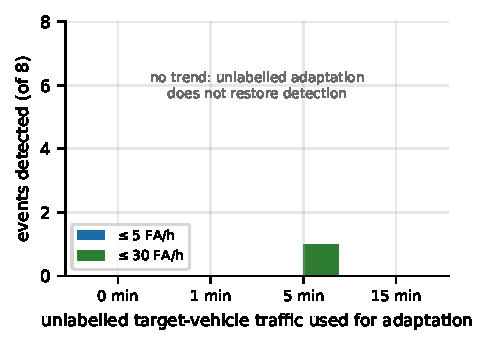
\includegraphics[width=0.52\linewidth]{figs/adaptation.pdf}
\caption{Unlabelled adaptation does not repair transfer. The source-trained detector is given 0, 1,
5 or \SI{15}{\minute} of the target vehicle's attack-free traffic (identifiers added to the
vocabulary, frames added as negatives, threshold calibrated on a held-out fifth), and evaluated on
target attack captures never used for adaptation.}
\label{fig:adapt}
\end{figure}

Figure~\ref{fig:adapt} shows that supplying unlabelled traffic from the target vehicle does not
help: 0 or 1 of 8 events at a valid operating point, with no trend in the amount of traffic. The
mechanism is visible in the construction: those identifiers' embeddings are trained exclusively on
normal traffic, so the classifier has never seen what an attack looks like on any of them.

\subsection{Identifier-agnostic representations transfer}

Table~\ref{tab:cross} reports the alternative. Both identifier-agnostic representations transfer
across all four pairs with no labels from the target vehicle: the per-frame relative representation
$\phirel$ detects 34.3 of 44 unknown-vehicle events (78\%) and the residualisation representation
$\phires$ 30.3 of 44 (69\%), against 0 of 44 for identifier embeddings. Transfer is therefore a
property of identifier-agnostic representations in general rather than of one particular feature
set, which also means that the representation of \citet{hegde2026residualization}, published without
a cross-vehicle evaluation, transfers.

The two differ in their blind spots, and complementarily so: on masquerade attacks $\phires$ reaches
40\% against 18\% for $\phirel$. Concatenating them into a single 26-feature input fails --
unknown-vehicle detection drops to 53\% at \SI{5}{\per\hour} and 60\% at \SI{30}{\per\hour}, and on
one pair the combined model collapses to 0 of 10 because its scores on the target vehicle's clean
traffic saturate near 1.0 so that no threshold satisfies the budget, while with the source vehicle's
threshold it still finds 10 of 10. Discrimination survives; calibration does not. Complementary
representations must therefore be combined as separate detectors, which is what Section~\ref{sec:pair}
does.

\begin{table}[t]
\centering
\caption{Cross-vehicle detection at $\leq$\SI{5}{\per\hour}, thresholds calibrated on the target
vehicle's own attack-free traffic, three seeds. Three of the four pairs cross manufacturers.}
\label{tab:cross}
\small
\begin{tabular}{lrrrr}
\toprule
Vehicle pair & Events & ID embedding & $\phires$ residualisation & $\phirel$ relative\\
\midrule
Impala $\rightarrow$ Silverado   & 8  & 0 & $2.7\pm0.5$  & $\mathbf{6.3\pm1.7}$\\
Traverse $\rightarrow$ Forester  & 12 & 0 & $\mathbf{12.0\pm0.0}$ & $\mathbf{12.0\pm0.0}$\\
Silverado $\rightarrow$ Forester & 10 & 0 & $\mathbf{10.0\pm0.0}$ & $\mathbf{10.0\pm0.0}$\\
Forester $\rightarrow$ Traverse  & 14 & 0 & $5.7\pm0.5$  & $\mathbf{6.0\pm0.0}$\\
\midrule
Total                            & 44 & 0 (0\%) & 30.3 (69\%) & \textbf{34.3 (78\%)}\\
Masquerade subsets               & 26 & -- & \textbf{10.3 (40\%)} & 4.7 (18\%)\\
\bottomrule
\end{tabular}
\end{table}

\section{Paired identifier-agnostic detectors}
\label{sec:pair}

\begin{figure}[t]
\centering
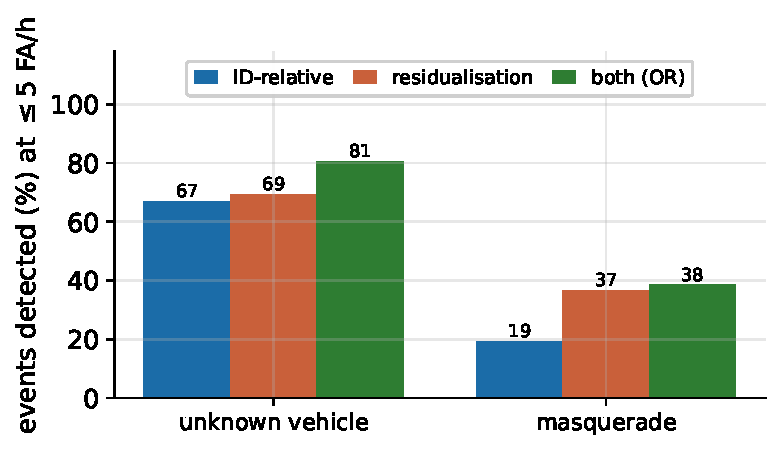
\includegraphics[width=0.60\linewidth]{figs/pair_union.pdf}
\caption{Two identifier-agnostic detectors with OR-ed alarms, each calibrated to half the budget, on
the unknown vehicle and on masquerade attacks (four pairs $\times$ two seeds, $\leq$\SI{5}{\per\hour}).
The union exceeds both branches on both test sets.}
\label{fig:pair}
\end{figure}

\begin{table}[t]
\centering
\caption{Paired detector on can-train-and-test, four vehicle pairs $\times$ two seeds. Unknown
vehicle: 88 events; masquerade: 52 events. Each branch of the union is calibrated to $B/2$.}
\label{tab:pair}
\begin{tabular}{lrrrrr}
\toprule
& \multicolumn{2}{c}{Unknown vehicle} & \multicolumn{2}{c}{Masquerade} & \\
\cmidrule(lr){2-3}\cmidrule(lr){4-5}
Branch & $\leq$\SI{5}{\per\hour} & $\leq$\SI{30}{\per\hour} & $\leq$\SI{5}{\per\hour} &
$\leq$\SI{30}{\per\hour} & Measured FA/h\\
\midrule
A: $\phirel$ relative        & 59/88 (67\%) & 62/88 (70\%) & 10/52 (19\%) & 16/52 (31\%) & 1.2\\
B: $\phires$ residualisation & 61/88 (69\%) & 63/88 (72\%) & 19/52 (37\%) & 25/52 (48\%) & 1.3\\
A $\vee$ B                   & \textbf{71/88 (81\%)} & \textbf{73/88 (83\%)} &
\textbf{20/52 (38\%)} & \textbf{27/52 (52\%)} & \textbf{0.3}\\
\bottomrule
\end{tabular}
\end{table}

Because the blind spots are disjoint, we run both representations as separate detectors and raise an
alarm when either fires. Table~\ref{tab:pair} and Figure~\ref{fig:pair} report the result. The union
detects 71 of 88 unknown-vehicle events (81\%) at \SI{0.3}{\per\hour} measured false alarms, against
67\% and 69\% for the branches alone at 1.2--\SI{1.3}{\per\hour}, and 83\% at a \SI{30}{\per\hour}
budget. On masquerade attacks it reaches 38\% at \SI{5}{\per\hour} and 52\% at \SI{30}{\per\hour},
roughly double the relative branch alone. The union improves detection \emph{and} lowers the
measured false-alarm rate, because each branch operates at a stricter threshold; it is therefore not
a trade-off between the two objectives. Masquerade coverage of 38--52\% remains the principal open
problem and is consistent with the contextual tier being the hardest case throughout this study.

Operationally the design degrades gracefully. On a vehicle with no labelled attacks, both branches
are available because neither requires target labels -- only the \SI{30}{\second} warm-up and a
short attack-free recording for calibration. If labelled attacks for that vehicle later become
available, a vehicle-specific branch can be added to the same disjunction without changing the
calibration procedure.

\section{Ablation study}
\label{sec:ablation}

\begin{figure}[t]
\centering
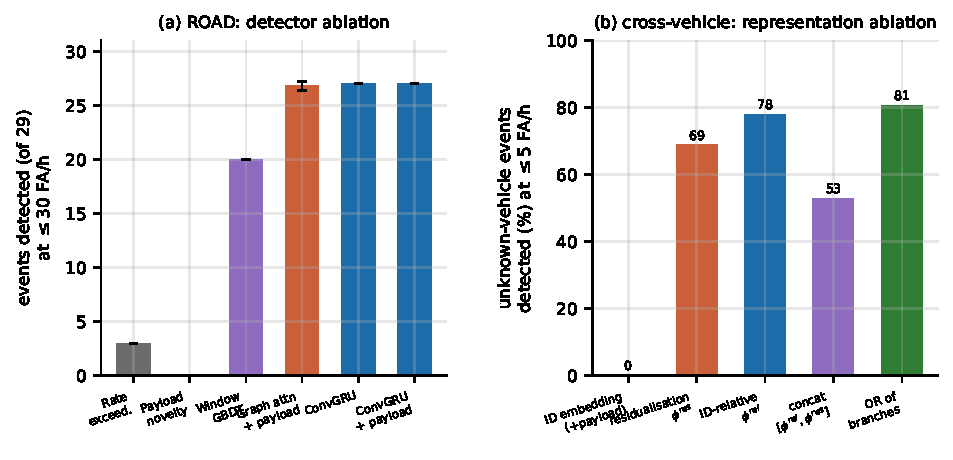
\includegraphics[width=\linewidth]{figs/ablation.pdf}
\caption{(a) Detector ablation on ROAD at $\leq$\SI{30}{\per\hour}: removing history and the graph
(GBDT) costs seven events, while replacing the graph model with a ten-times smaller ConvGRU costs
nothing. (b) Representation ablation on can-train-and-test: identifier embeddings transfer to
nothing, both identifier-agnostic representations transfer, concatenating them is worse than either,
and running them as two detectors is best.}
\label{fig:ablation}
\end{figure}

\begin{table}[t]
\centering
\caption{Ablations. Upper block: detector components on ROAD (29 events, $\leq$\SI{30}{\per\hour}).
Lower block: representation and combination on can-train-and-test (44 unknown-vehicle events,
$\leq$\SI{5}{\per\hour}). $\Delta$ is the change with respect to the row marked as reference.}
\label{tab:ablation}
\small
\begin{tabular}{llrr}
\toprule
Ablation & Configuration & Events & $\Delta$\\
\midrule
\multirow{5}{*}{ROAD detector}
 & ConvGRU + payload novelty (reference) & $27.0\pm0.0$ & --\\
 & $-$ payload novelty (raw frames only) & $27.0\pm0.0$ & $0.0$\\
 & $+$ graph attention, $10\times$ parameters & $26.8\pm0.4$ & $-0.2$\\
 & $-$ temporal history, $-$ sequence model (window GBDT) & $20.0$ & $-7.0$\\
 & $-$ supervision (payload novelty exceedance) & $0.0$ & $-27.0$\\
\midrule
\multirow{5}{*}{Cross-vehicle}
 & $\phirel$ relative (reference) & 34.3 (78\%) & --\\
 & $\phires$ residualisation & 30.3 (69\%) & $-4.0$\\
 & identifier embedding $+$ payload & 0.0 (0\%) & $-34.3$\\
 & concatenation $[\phirel,\phires]$ & 23.3 (53\%) & $-11.0$\\
 & two detectors, OR-ed alarms & \textbf{81\% of 88 events} & $+3$\,pp\\
\bottomrule
\end{tabular}
\end{table}

Table~\ref{tab:ablation} and Figure~\ref{fig:ablation} summarise the ablations; the last row of each
block is the configuration we recommend.

On ROAD (upper block), removing the payload-novelty features from the ConvGRU costs nothing at this
budget, and adding graph attention with ten times the parameters also changes nothing within noise.
Removing the temporal history and the sequence model -- the window GBDT, which sees all identifiers
of the current window but no past -- costs seven events, which locates the useful signal in the
short-term temporal structure rather than in the cross-identifier graph. Removing supervision
altogether costs everything at a usable budget: the unsupervised novelty test detects no events at
\SI{30}{\per\hour}, despite finding every value attack when its threshold is tuned for window-$F_1$
(Fig.~\ref{fig:latency}b). That contrast is itself a warning about window-level metrics.

Across vehicles (lower block), the representation is decisive. Identifier embeddings lose all 34
events that $\phirel$ recovers. Residualisation recovers most of them, confirming that the property
that matters is the absence of identifier identity rather than our particular features.
Concatenation loses eleven events relative to $\phirel$ despite containing strictly more information,
because the joint input degrades score calibration on unseen vehicles. Running the two
representations as separate detectors recovers three percentage points over the better branch while
halving the measured alarm rate.

\section{Deployment cost}
\label{sec:cost}

\begin{table}[t]
\centering
\caption{Inference cost, one CPU thread, batch size 1. ``Rate'' is the number of inferences per
second implied by the sliding-window stride; ``duty'' is the resulting fraction of one core.}
\label{tab:cost}
\begin{tabular}{lrrrrrr}
\toprule
Model & Params & int8 & Median & p99 & Rate & Duty of one core\\
\midrule
ConvGRU + payload novelty      & 98\,k   & 0.10\,MB & \SI{1.35}{\milli\second} & \SI{1.69}{\milli\second} & \SI{150}{\per\second} & 20\%\\
Graph attention                & 1.05\,M & 1.05\,MB & \SI{38.9}{\milli\second} & \SI{70.1}{\milli\second} & \SI{10}{\per\second} & 39\%\\
Graph attention, 50 MC passes  & 1.05\,M & 1.05\,MB & \SI{1945}{\milli\second} & \SI{3507}{\milli\second} & \SI{10}{\per\second} & 1945\%\\
\midrule
Paired detector (two ConvGRU)  & 196\,k  & 0.20\,MB & \SI{2.70}{\milli\second} & \SI{3.38}{\milli\second} & \SI{150}{\per\second} & 40\%\\
\bottomrule
\end{tabular}
\end{table}

Table~\ref{tab:cost} reports measured inference cost. The 98\,k-parameter detector needs 0.10\,MB in
int8 and about 20\% of one core at the rate implied by its stride; the paired design of
Section~\ref{sec:pair} doubles both. Feature extraction adds 0.3\% of a core over real traffic and is
negligible. By contrast, the 50-pass Monte-Carlo-dropout uncertainty estimate that accompanies much
of the forecasting literature \citep{gal2016dropout} requires roughly twenty cores at the same window
rate, which rules it out for an embedded deployment; five passes, or a deterministic calibration
method, would be needed instead. A laptop core is several times faster than a typical automotive
Cortex-A or Cortex-R core, so these figures are optimistic lower bounds; the duty column is the
quantity that scales with a slower core.

\section{Discussion}
\label{sec:discussion}

\paragraph{Benchmark accuracy has stopped being informative.} Two of our corpora are saturated at the
window level: on Car-Hacking every model we tried reaches AUC 1.000, and on ROAD every learned model
reaches the same 27-of-29 ceiling. Under those conditions, differences between published $F_1$
scores in the third decimal place carry no information about deployability, while quantities that do
-- alarms per hour, behaviour on an unseen vehicle, cost on a real core -- are rarely reported
(Table~\ref{tab:related-eval}). Our results suggest reallocating effort from architecture to
evaluation and representation.

\paragraph{Why complexity does not pay here.} The graph-attention model was designed on the
assumption that cross-identifier structure carries attack evidence. Figure~\ref{fig:latency}b shows
that the assumption is correct for contextual attacks, but Table~\ref{tab:ablation} shows that a flat
model over all identifiers already captures it; what the graph adds beyond that is within seed noise.
Meanwhile, the ablation that does matter -- removing temporal history -- costs seven events. On the
evidence here, temporal structure and a sensible representation are the load-bearing components.

\paragraph{The vehicle gap is a representation problem.} The most consequential finding for practice
is that a detector which scores well on its own vehicle can detect nothing on another while appearing
to work, because the alarm simply never clears. Identifier embeddings are the cause: they tie the
model to a vocabulary that does not survive the change of vehicle, and they cannot be repaired with
unlabelled traffic because the new identifiers are only ever seen in normal traffic. Once the
representation is expressed relative to each identifier's own behaviour, most of the detection
returns. This also implies a practical commissioning procedure: record half an hour of ordinary
driving from a new vehicle model, calibrate thresholds on it, and deploy -- no labelled attacks
required.

\paragraph{What remains hard.} Masquerade attacks are the residual problem: 38--52\% coverage with
the paired design, and 0 of 12 for a per-identifier novelty test on ROAD's contextual attacks. They
are hard for a principled reason -- every frame is individually plausible -- and they are exactly the
attacks that matter most for a capable adversary. Progress here will require models of the
consistency between signals carried by different identifiers, evaluated under the protocol used
here rather than at a window-$F_1$ optimum.

\paragraph{Threats to validity.} Our conclusions rest on three public corpora, one of which supplies
all cross-vehicle evidence; a fifth vehicle pair could change the numbers, though it is unlikely to
restore identifier-embedding transfer given the mechanism. Our re-implementations of a
residualisation representation and of frame-sequence baselines follow published descriptions rather
than authors' code, so absolute values may differ from the originals; we therefore draw conclusions
only from comparisons run within our own protocol, and we release the code so that the comparison can
be repeated. Seed variance is substantial at strict budgets, which is why every learned result is
reported over three to five seeds with a statistical test. Finally, all timings come from one laptop
CPU and are bounds rather than automotive measurements.

\section{Reproducibility}
\label{sec:repro}

All code, configurations, evaluation harness and result summaries are available at
\url{https://github.com/shishirbit/can-ids-evaluation}. The repository contains the dataset
preparation scripts (\texttt{scripts/preprocess\_*.py}, \texttt{scripts/download\_*.sh}), the
detectors (\texttt{src/galaxy\_its/models/}), the identifier-agnostic representations
(\texttt{src/galaxy\_its/data/relative.py}, \texttt{residual.py}), the evaluation harness
(\texttt{src/galaxy\_its/eval/operating.py}), the experiment drivers
(\texttt{scripts/train\_sttf.py}, \texttt{baseline\_frames.py}, \texttt{id\_agnostic.py},
\texttt{cross\_vehicle.py}, \texttt{per\_vehicle\_calib.py}, \texttt{pair\_detector.py}), the
statistical comparison (\texttt{scripts/compare\_models.py}) and the figure generators
(\texttt{scripts/make\_figures.py}, \texttt{make\_figures2.py}). Every number quoted in this paper is
recorded in \texttt{experiments/paper\_numbers.json} together with the script that produced it, and
the figures are generated from that file so that text, tables and plots cannot diverge.

The raw corpora are not redistributed: Car-Hacking and ROAD are obtained from their authors and
can-train-and-test from its repository, using the download scripts provided. A full replication
requires approximately 11\,GB of disk for the corpora, a CUDA-capable GPU with 8\,GB of memory, and
about 12 hours of compute for all experiments reported here; individual experiments take 3--20
minutes. Random seeds, hyperparameters and split definitions are fixed in the experiment drivers and
recorded in each run's \texttt{results.json}.

\section{Conclusion and future work}
\label{sec:conclusion}

We have argued, and measured, that the quantities deciding whether a CAN intrusion detector can be
deployed are not benchmark accuracies but the number of attack events caught per hour of false
alarms and the behaviour of the detector on a vehicle it has not seen. Under an event-level protocol
with an explicit false-alarm budget and an alarm duty cap, the most widely used benchmark turns out
to reward learning an injection timetable; a 98\,k-parameter model matches a 1.05\,M-parameter one on
the hardest public corpus, both stopping at a ceiling imposed by the data; five evaluation choices
each reverse model rankings; and identifier-embedding detectors, the standard design, detect nothing
on an unseen vehicle at a usable alarm rate. Expressing each frame relative to its own arbitration
identifier restores 69--78\% of that detection without any labels from the target vehicle, and
running two such representations as separate detectors with OR-ed alarms reaches 81\% at
\SI{0.3}{\per\hour} false alarms for 0.20\,MB of parameters and roughly 40\% of one CPU core.

Future work follows directly from what remains hard. First, masquerade and other contextual attacks
need explicit models of cross-identifier signal consistency; the tier analysis here gives a concrete
target and a way to measure progress. Second, the protocol should be extended to suppression
attacks, which remove frames rather than adding them and therefore need a different notion of
episode. Third, the cross-vehicle study should be repeated on a fleet-scale corpus with more than
four vehicles, ideally including vehicles from a third manufacturer. Finally, we recommend that
future CAN IDS results be reported at a stated false-alarm budget, with an alarm duty cap, on whole
held-out drives, and -- wherever the data permit -- on a vehicle the detector has never seen.

\section*{Declaration of competing interest}
The authors declare that they have no known competing financial interests or personal relationships
that could have appeared to influence the work reported in this paper.

\section*{CRediT authorship contribution statement}
\textbf{First Author}: Conceptualization, Methodology, Software, Investigation, Data curation,
Writing -- original draft. \textbf{Second Author}: Validation, Formal analysis, Writing -- review \&
editing. \textbf{Third Author}: Supervision, Project administration, Writing -- review \& editing.

\section*{Data availability}
The three corpora used are public and are obtained from their original providers; the code and
result summaries are available at \url{https://github.com/shishirbit/can-ids-evaluation}.

\bibliographystyle{elsarticle-harv}
\bibliography{refs}

\end{document}
